\subsection{Objectives}

The purpose of the experiment is to show the following points:
\begin{itemize}
\item the learning engine produces *accurate* and *concise* descriptions compared to a human
expert's descriptions but costs just a fraction of the time; 
\item it handles a variety of data formats; 
\item the refinement step significantly improves the structure; 
\item it is able to produce a description that is sufficiently accurate with 
much smaller training sets (overfitting vs. underfitting); 
\item demonstrate that there exists a correlation between sample size, execution time and accuracy,
and the min sample size required to achieve certain accuracy correlates with the 
data complexity.
\end{itemize}

\subsection{Setup}
\begin{table*}
\begin{center}
\begin{tabular}{|c|c|c|c|c|c|c|c|c|} \hline
Title		& Chunks & Bytes	& Mode  &Header	& Array	& Group & Msgs 	& Comments \\ \hline \hline
1967Transactions.short	& 999	& 70929	& line	& no	& no	& no	& no	& transaction records \\ \hline
MER\_T01\_01.cvs	& 491	& 21731 & line  & yes	& no	& yes	& no	& comma-separated records\\ \hline
ai.3000		& 3000		& 293460 & line	& no	& no	& yes	& no	& web log of Amnesty International \\ \hline
asl.log &	1500	& 279600	& line	& no	& no	& yes	& no	& log file of Mac ASL \\ \hline	
boot.log	& 262	& 16241		& line	& no	& no	& no	& yes	& Mac OS boot log \\ \hline
crashreporter.log	& 441	& 50152 & line	& no	& no	& no	& yes	& crashreporter daemon log \\ \hline
crashreporter.mod & 441	& 49255	& line	& no	& no	& no	& yes	& modified crashreporter daemon log \\ \hline
dibbler.1000	& 999	& 142607 	& line	& yes	& yes	& no	& no	& AT\&T call log \\ \hline
ls-l.txt	& 35	& 1979		& line	& yes	& no	& no	& no	& Stdout from Unix command ls -l \\ \hline
netstat-an	& 202	& 14355		& block	& yes	& no	& no	& no	& output from netstat -an \\ \hline
page\_log	& 354	& 28170		& line	& no	& no	& no	& no	& printer logs \\ \hline
quarterlypersonalincome & 62	& 10177	& line	& yes	& no	& yes	& no	& spread sheet \\ \hline
railrail.txt	& 67	& 6218		& line	& yes	& no	& yes	& no	& US rail road info \\ \hline
scrollkeeper.log & 671	& 66288		& line	& no	& no	& no	& yes	& log from cataloging system \\ \hline
windowserver\_last.log & 680	& 52394	& line	& no	& no	& no	& yes	& log from LoginWindow server on Mac \\ \hline
yum.txt		& 328	& 18221		& line	& no	& no	& no	& no	& log package installer Yum \\ \hline
\end{tabular}
\caption{Benchmark profile}
\end{center}
\end{table*}

\begin{enumerate}
\item Brief intro to 15 golden formats in a big table and possibly group them by
features

\item Machine profile: Apple PowerBook G4, 1.67 GHz, 512 MB DDR ram running on 
Mac OS X 10.4 Tiger. 

\item Experiment parameter: data size (num of records and byte count), accuracy (success rate of parsing), 
timing (human time vs. machine time), structure quality (normalized scores), sample size

\item Different representations: HW IR, HW PADS, Inferred IR, Inferred PADS, we measure
the accuracy on the HW PADS and inferred PADS, and the time to produce and the MDL scores on
the HW IR and inferred IR.

\begin{table}
\begin{center}
\begin{tabular}{|l|c|c|c|} \hline
		& Parsing accuracy 	& MDL score 	&  Time to prod.\\ \hline
Inferred IR 	& -			& X		& X	\\ \hline
Inferred PADS	& X			& -		& -	\\ \hline 
Human IR	& -			& X		& X	\\ \hline	
Human PADS	& X			& -		& -	\\ \hline	
\end{tabular}
\caption{Relationship between representations and measurements}
\end{center}
\end{table}

\end{enumerate}

\subsection{Experiments}

\begin{enumerate}
\item Human expert coded IR for all 12 formats: measure timing, score of the structure and assume 100\% 
accuracy. This is the control data.

\item Run learning tool on all 12 data files in full length: measure timing for structure discovery, 
and refinement; initial scores and final scores, parsing rate (should be all 100\%).
For accurate timing measurements, run each data format 10 times, and take average after removing the
best and the worst time.
Compare these with the golden numbers from (1) in a big table. Show that the difference in scores
can be siginificant in some cases hence room for improvement (may go into the discussion section)
but timing advantage is huge and refinment improves initial struct a lot. Maybe also compare a case or
two where the score from silver is comparable to golden and the actually description produced is also
close to golden (to demo that our scoring makes some sense).
Have a discussion here about while the learning tool may produce a longer description than human does,
it parses all data correctly so the user is getting all these for free which is a tremendous benefit.
Discuss 1967 where the inference does better than human.

\begin{table*}
\begin{center}
\begin{tabular}{|l||r|r|r||r|r|r|c|} \hline
Formats 	& Inf score 	&Ref score	& Man score 	& Inf time 	& Ref time 	& Total time  	& Man time (h)\\ \hline \hline
1967Transactions.short & 0.295 	&0.218 		&0.268		& 0.22       	& 2.08     	& 2.30  	& 4.0  \\ \hline
MER\_T01\_01.csv & 0.648 	&0.112		&0.138		& 0.11       	& 2.61       	& 2.72 		& 0.5  \\ \hline
ai.3000          & 0.503	&0.332		&0.338		& 2.02       	& 27.36      	& 29.38		& 1.0  \\ \hline
asl.log          & 0.630	&0.267		&0.361		& 2.91       	& 613.01	& 615.92 	& 1.0  \\ \hline
boot.log         & 0.620	&0.481		&0.703		& 0.12       	& 5.81       	& 5.92 		& 1.0  \\ \hline
crashreporter.log & 0.607	&0.328		&0.348		& 0.13       	& 5.47       	& 5.59 		& 2.0  \\ \hline
crashreporter.log.mod & 0.612	&0.329		&0.347		& 0.15       	& 5.76       	& 5.90 		& 2.0  \\ \hline
dibbler.1000     & 0.602	&0.470		&0.438		& 2.15       	& 8.22       	& 10.36 	& 0.5  \\ \hline
ls-l.txt         &0.559		&0.333		&0.401		& 0.01       	& 0.14       	& 0.14 		& 1.0  \\ \hline
netstat-an       &0.413		&0.394		&0.319		& 0.05       	& 3.26       	& 3.32 		& 1.0  \\ \hline
page\_log        & 0.540	&0.107		&0.353		& 0.12       	& 0.47       	& 0.59 		& 0.5   \\ \hline
quarterlypersonalincome & 0.544	&0.367		&0.354		& 0.06       	& 15.87      	& 15.93 	& 48  \\ \hline
railroad.txt     &0.715		&0.506		&0.522		& 0.05       	& 22.70      	& 22.75 	& 2.0  \\ \hline
scrollkeeper.log & 0.625	&0.354		&0.352		& 0.11       	& 4.46       	& 4.57 		& 1.0  \\ \hline
windowserver\_last.log &0.618	&0.241		&0.267		& 0.31       	& 18.57      	& 18.88 	& 1.5  \\ \hline
yum.txt          &0.827		&0.305		&0.474		& 0.10       	& 1.92       	& 2.02 		& 5.0  \\ \hline
\end{tabular}
\caption{Golden results (Inf: structure inference, Ref: Refinement, Man: Human expert)}
\end{center}
\end{table*}

\item Select random training sets of 5\%, 10\%, 15\%, 20\% 25\%, 30\%, 35\% and 40\% of 
the original data (3 sets for each size) and run learning tool end to end on 
them and take the average of 3 sets. 
Set a threshhold level of 95\% accuracy and record how much training data (in percentage and
absolute terms) is needed for each golden format to achieve this accurary. Then relate this
to the normalized type complexty of the inferred IR of the entire data sets.
Plot graph of (timing, accuracy) vs. training size 
for a few examples, and show that we are doing a good job with reasonable sample size. The diagram should
show increasing accuracy and execution time as sample size goes up. Point out anomaly
where the abolute training size is too small (e.g. for ls-l.txt which only has 35 lines) which results
in overfitting. ls-l.txt is also problematic as it has a header in the first line and if that is not included
in the training set, the data will not parse.

\begin{figure}
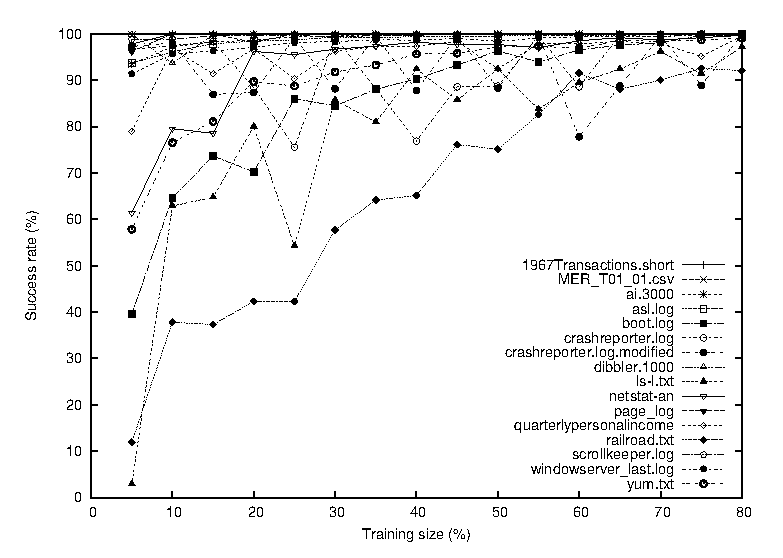
\epsfig{file=successrate.eps, width=\columnwidth}
\caption{Success rates of training sets}
\end{figure}

\begin{figure}
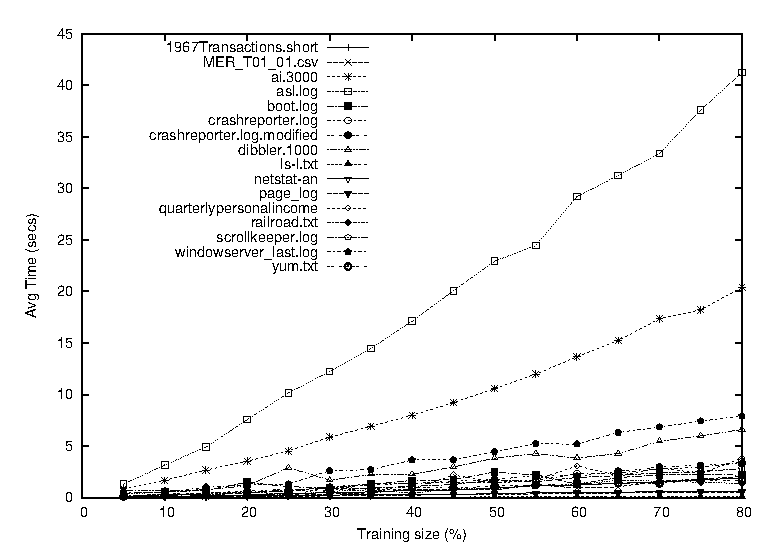
\epsfig{file=traintime.eps, width=\columnwidth}
\caption{Execution times of training sets}
\end{figure}
\end{enumerate}

\begin{table}
\begin{center}
\begin{tabular}{|c|r|l|c|c|} \hline
Title 			& Bytes 	& Ty Comp	& 90\% 		& 95\% \\ \hline \hline
1967Transactions.short	& 70929		& 0.0003	& 5		& 5 			\\ \hline
MER\_T01\_01.csv        & 21731 	& 0.0037	& 5		& 5\\ \hline
ai.3000                 & 293460 	& 0.0004	& 5		& 10\\ \hline
asl.log                 & 279600	& 0.0012	& 5		& 10\\ \hline
boot.log                & 16241		& 0.0213	& 40		& 50\\ \hline
crashreporter.log       & 50152 	& 0.0052	& 5		& 5\\ \hline
crashreporter.log.mod   & 49255		& 0.0053	& 5		& 5\\ \hline
dibbler.1000            & 142607 	& 0.0001	& 5		& 5\\ \hline
ls-l.txt                & 1979		& 0.0461	& 50		& 70\\ \hline
netstat-an              & 14355		& 0.0118	& 20		& 25\\ \hline
page\_log               & 28170		& 0.0032	& 5		& 5\\ \hline
quarterlypersonalincome & 10177		& 0.017		& 10		& 20\\ \hline
railroad.txt            & 6218		& 0.0485	& 60		& 85\\ \hline
scrollkeeper.log        & 66288		& 0.002		& 5		& 5\\ \hline
windowserver\_last.log  & 52394		& 0.0084	& 5		& 10\\ \hline
yum.txt                 & 18221		& 0.0124	& 30		& 40\\ \hline
\end{tabular}
\caption{Min Training size (\%) vs. required accuracy}
\end{center}
\end{table}

\begin{figure}
\begin{center}
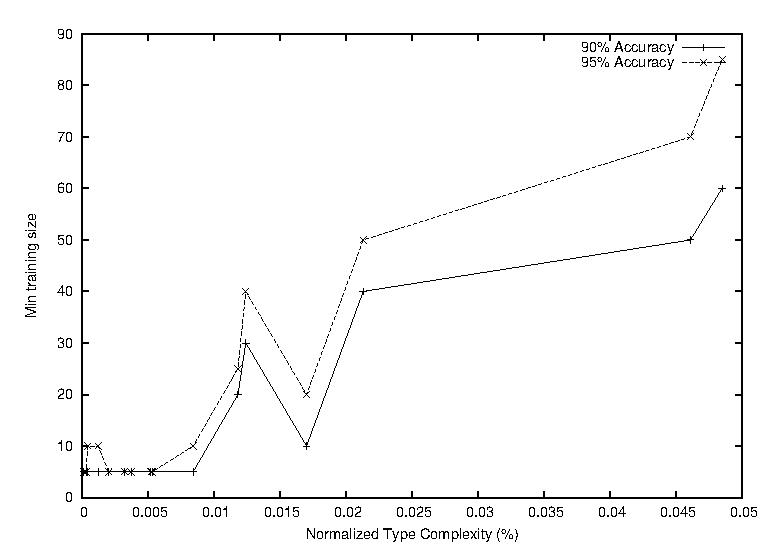
\epsfig{file=traintycomp.eps, width=\columnwidth}
\caption{Correlation between structure complexity of 
the data and minimum training size required}
\end{center}
\end{figure}
